%Folgende Zeile aktivieren und als SVN property "svn:keywords" auf "Id" setzen, um SVN Versionsinformationen im Dokument zu erhalten
%\svnInfo $Id: einleitung.tex 60 2012-01-26 15:56:06Z koppor $ 

\chapter{3D - Verfahren}
\label{chap:3d}
\subsection{RANSAC}
RANSAC (\textbf{RA}ndom \textbf{SA}mple \textbf{C}onsensus) ist ein iteratives Verfahren zur Schätzung eines mathematischen Models anhand von Beobachtungsdaten mit Ausreißern. Der Algorithmus ist nicht-deterministisch, da ihm probabilistische Ansätze zu Grund liegen. Aufgrund seiner Robustheit wird er häufig im Bereich des maschinellen Sehens eingesetzt. 

\begin{figure}[H]
  \begin{center}
    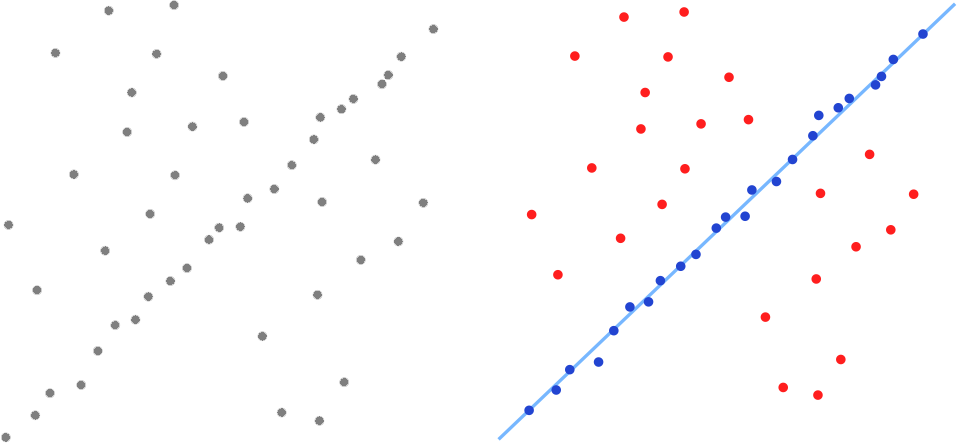
\includegraphics[width=0.9\textwidth]{RANSACline.png}
    \caption{In einen Datensatz mit vielen Ausreißern wird eine Linie eingepasst.}
    \label{fig:l_alg_1}
  \end{center}
\end{figure}

\subsection{Der Algorithmus}
 Für das zu erkennende Objekt wird ein parameterabhäniges Modell erstellt. Danach werden die Daten iterativ auf mögliche Vorkommnisse eines auf das Modell passenden Objekts getestet, dafür werden iterativ zufällige Punkte aus den Daten selektiert und als hypothetische Einlieger des Objekts betrachtet und das Modell an diese Punkte angepasst. Für eine Linie wären dies zwei Punkte um sie ausreichend zu beschreiben. Nun wird das Modell getestet:

\begin{enumerate}
\item Alle anderen Punkte werden gegen das Modell getestet und falls sie dazu passen ebenfalls als mögliche Einlieger gespeichert.
\item Das Modell wird akzeptiert wenn genug Einlieger gefunden werden.
\item Das Modell auf Basis aller gefundenen Einlieger neu berechnet und evaluiert.
\end{enumerate}

Nach ausreichend vielen Iterationen wird das beste Modell benutzt um alle Punkte des Objekts zu identifizieren. Anschließend wird das gefundene Objekt aus den Daten gelöscht und gegebenenfalls nach weiteren Vorkommnissen gesucht.

\begin{figure}[H]
  \begin{center}
    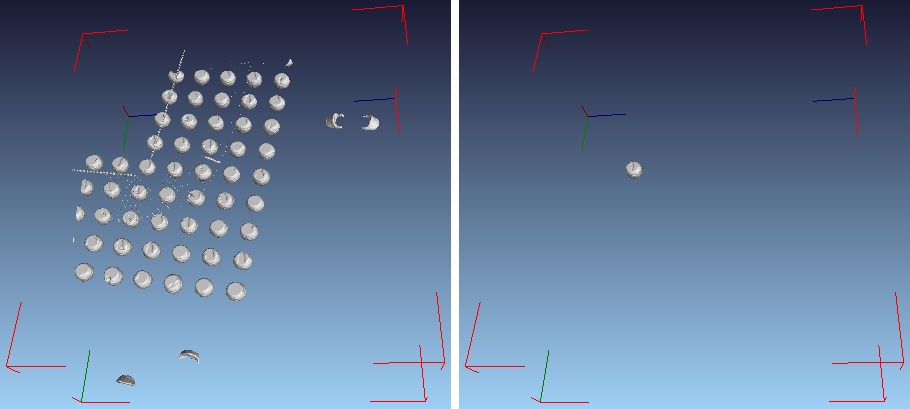
\includegraphics[width=0.9\textwidth]{RANSACball.png}
    \caption{In einem per Threshhold-Verfahren vorverarbeiteten Datensatz wird anhand eines einfachen Modells eine Kugel identifiziert.}
    \label{fig:l_alg_1}
  \end{center}
\end{figure}

\subsection{Bewertung}
Der Algorithmus eignet sich sehr gut um in großen Datenmengen schnell Instanzen von Modellen zu finden. Für den diskutierten Anwendungsfall ist er leider vergleichsweise langsam. Der Grund dafür ist, dass die zu suchenden Objekte schon durch einen Dichte-Threshhold sehr gut vor-isoliert werden können. Man kann sich deshalb direkt darauf konzentrieren einzelne Punktmengen auf bestimmte Eigenschaften hin zu untersuchen. Der große Vorteil von RANSAC schnell mögliche Kandidaten zu entdecken wird deshalb negiert.